\documentclass[13pt,a4paper]{report}
\usepackage[utf8]{}
\usepackage{fancybox}
\usepackage[margin=0.85in]{geometry} 
\usepackage{amsmath, amsthm, amssymb,latexsym,amscd,amsfonts,enumerate}
\usepackage{tabularx}
\usepackage{indentfirst}
\usepackage{float}
\usepackage{enumitem}
\usepackage[nottoc]{tocbibind}
\PassOptionsToPackage{hyphens}{url}
\usepackage{hyperref}
\usepackage{afterpage}
\usepackage[square,numbers]{natbib}
\usepackage{chngcntr}
\usepackage[super]{nth}
\usepackage{titlesec}
\usepackage{gensymb}
\usepackage{chemmacros}
\usepackage{multirow}
\usepackage{pgfplots}
\usepackage{tikz}
\usepackage{bigdelim}
\usepackage{tocloft}
\usepackage{minted}

\usepackage[
backend=biber,
% style=alphabetic,
sorting=none,
]{biblatex}
\addbibresource{references.bib} %Imports bibliography file
% \DeclareFieldFormat{labelnumber}{\the\numexpr#1+1\relax}

\usepackage[utf8]{inputenc}
\usepackage[vietnamese,main=english]{babel}

\usepackage{makecell}

\renewcommand\labelitemi{$-$}

\titleformat{\chapter}[display]
  {\normalfont\bfseries}{}{0pt}{\Huge}
  
\renewcommand*\thesection{\textbf{\Roman{section}}}
\renewcommand*\thesubsection{\arabic{subsection}.}


% SECTION FORMAT
\titleformat{\section}%[display]
{\normalfont\bfseries\fontsize{22}{26}\selectfont\raggedright}% Format and bigger size of title text with boldface
{\llap{%
    \rule[-6pt]{3cm}{1.3cm}\rule{6pt}{0pt}}% Black box to the left, lowered 6pt. The end rule is a horisontal space.
  \llap{% Number also to the left, on top of the black box, with bigger font size as section title.
    \fontsize{22}{26}\selectfont\color{white}\thesection\rule{10pt}{0pt}}}
{0pt}
{}{}
\titlespacing*{\section}
  {0pt}{40pt}{10pt}



\renewcommand{\bottomtitlespace}{0cm}

\newcolumntype{Y}{>{\centering\arraybackslash}X}
\renewcommand\tabularxcolumn[1]{m{#1}}

\newcommand\blankpage{%
    \null
    \thispagestyle{empty}%
    \addtocounter{page}{-1}%
\newpage}

\usepackage[none]{hyphenat}
\sloppy % accept really ugly paragraphs

\usepackage{tcolorbox}
\usepackage{etoolbox}
\BeforeBeginEnvironment{minted}{\begin{tcolorbox}}%
\AfterEndEnvironment{minted}{\end{tcolorbox}}%
\renewcommand{\theFancyVerbLine}{\sffamily \textcolor[rgb]{0.5,0.5,1.0}{\normalsize {\arabic{FancyVerbLine}}}}

\setminted{
  framesep=2mm,
  linenos=true,
  breaklines,
  breakanywhere,
  xleftmargin=10px,
  numbersep=7pt,
  escapeinside=||,
}
% \inputminted[texcomments]{python}{code/excerpt.py}
    
\titleformat{\chapter}[display]{\normalfont\huge\bfseries}{}{0pt}{\Huge}
\titleformat*{\subsubsection}{\large\bfseries}
\titlespacing*{\chapter}{0pt}{0pt}{0pt}
    
\newcolumntype{P}[1]{>{\centering\arraybackslash}p{#1}}
\newcolumntype{C}[1]{>{\centering\let\newline\\\arraybackslash\hspace{0pt}}m{#1}}
    
\setlist[itemize]{noitemsep, topsep=0pt}
\AtBeginEnvironment{multicols}{\RaggedRight}

\pagenumbering{roman}\pagestyle{plain}

\titlespacing*{\chapter}
{0pt}{-50pt}{0pt}

\begin{document}
%Trang bìa 1
\fontsize{13pt}{18pt}\selectfont
\begin{titlepage}
\thispagestyle{empty}
\thisfancypage{%đóng khung trang này
\setlength{\fboxsep}{0pt}% 8pt là độ dày của đường viền
\fbox}{} % phần nội dung sau là tương tự như đã làm
\

\begin{center}
% \vspace{-0.25cm}
\begin{large}
HO CHI MINH CITY UNIVERSITY OF TECHNOLOGY $-$ VNU HCMC
\end{large} \\
\begin{large}
OFFICE FOR INTERNATIONAL STUDY PROGRAM
\end{large} \\
\begin{large}
FACULTY OF APPLIED SCIENCE
\end{large} \\
\textbf{--------------------  $\ast$  ---------------------}\\[2.75cm]


\includegraphics[scale=1]{logoBK.png}\\[1cm]
{\fontsize{20pt}{1}\selectfont GENERAL PHYSICS 1}\\[1ex]
{\fontsize{20pt}{1}\selectfont MATLAB PROJECT REPORT}\\[2.75cm]
\end{center}

\begin{otherlanguage}{vietnamese}
\begin{tabbing}
	\hspace{2.35cm}Lecturers \ \ \ \ \ \ \ \ \ \ \ \=: \textbf{\parbox[t]{9cm}{Dr. Nguyễn Trung Hậu}}\\
 \> \ \ \textbf{\parbox[t]{9cm}{
		Dr. Nguyễn Xuân Thanh Trâm}} \\
	\hspace{2.35cm}Subject \>: \textbf{\parbox[t]{9cm}{General Physics 1}}\\
	\hspace{2.35cm}Class \>: \textbf{\parbox[t]{9cm}{CC03}}\\
	\hspace{2.35cm}Group \>: \textbf{\parbox[t]{9cm}{02}}\\
	\hspace{2.35cm}Members \>: \textbf{\parbox[t]{5.25cm}{
		Huỳnh Dương Gia Bảo}} \= $-$ 2252063 \\ \> \ \ \textbf{\parbox[t]{6cm}{
		Lương Triển Đạt}} \> $-$ 2252144 \\ \> \ \ \textbf{\parbox[t]{6cm}{
		Phạm Hoàng Quân}} \> $-$ 2252687 \\ \> \ \ \textbf{\parbox[t]{6cm}{
		Võ Minh Thăng 
  }} \> $-$ 2252762 \\
  \hspace{2.35cm}Completion date \>: \textbf{\parbox[t]{9cm}{May \nth{8}, 2023}}\\[12pt]
\end{tabbing}
\end{otherlanguage}

\vspace{0.35cm}
\begin{center}
{\fontsize{13pt}{1}\selectfont Ho Chi Minh City, May \nth{8}, 2023}
\end{center}
\end{titlepage}

\pagenumbering{gobble}


\setlength{\cftbeforetoctitleskip}{0em}
\setlength{\parindent}{1.75em} % indent hole text
\setlength{\cftbeforesecskip}{0.65em}
\setlength{\cftbeforesubsecskip}{0.65em}
\renewcommand\cftsecaftersnum{.}
\cftsetindents{section}{1.25cm}{3.5em}
\cftsetindents{subsection}{2.15cm}{1.35em}

\renewcommand{\cftchapfont}{\normalfont\LARGE\bfseries} % \chapter font in ToC
\renewcommand{\cftsecfont}{\normalfont\bfseries\LARGE}  % \section font in ToC
\renewcommand{\cftsubsecfont}{\normalfont\Large}     % \subsection font in ToC

\tableofcontents
\addtocontents{toc}{\vspace{-0.65cm}}

\pagenumbering{arabic}
\setcounter{page}{2}
\pgfkeys{
     /pgf/number format/precision=0, 
    /pgf/number format/fixed zerofill=true,
    /pgf/number format/fixed
}

% % Set section and subsection formatting
% \titleformat{\section}
%   {\normalfont\Large\bfseries}{\makebox[1.75em][l]{\thesection}}{0em}{}
\titleformat{\subsection}
  {\normalfont\Large\bfseries}{\hspace{-0.55cm}\makebox[1.25em][l]{\thesubsection}}{0em}{}

\pagenumbering{arabic}
\newpage
\setcounter{page}{2}
\section{Introduction}
The objective of this MATLAB project is to calculate and graphically represent the kinetic and potential energies of a particle moving under the influence of a conservative force. A conservative force is defined as a force whose work done on an object is independent of the path taken by the object, and depends only on its initial and final positions. In this project, we will consider a specific conservative force given by the expression: 
\begin{gather*}
F(x) = kx - 4qx^3\\
\text{where } k \text{ and } q \text{ are parameters}
\end{gather*}

To calculate the potential energy of the particle, we will integrate the force function with respect to position in order to obtain its value at any point along the particle's trajectory, i.e., $$U(x) = - \displaystyle \int F(x) dx$$

We will also calculate the kinetic energy of the particle, which is a function of its velocity, and hence of time. By combining the expressions for potential and kinetic energy, we can obtain the total mechanical energy of the particle, which is conserved for a conservative force.

Finally, we will use MATLAB to plot the functions for kinetic and potential energy as functions of time, along with the total mechanical energy. This will provide us with a graphical representation of the motion of the particle, which can help us to gain insights into its behavior under the influence of the conservative force.

\newpage
\section{Theory}
In this MATLAB project, we will use the Euler-Cromer method\cite{euler} to numerically compute the motion of a mass acted on by a conservative force. In the context of energy conservation, the total energy in the system (sum of kinetic and potential energies) is conserved for this type of motion. Specifically, the kinetic energy $K$ of the mass is given by the expression:
\begin{gather*}
K = \dfrac{1}{2}mv^2\\
\text{where } m \text{ is the mass, } v \text{ is the velocity}
\end{gather*}

Specifically, we will consider a potential energy function which has a corresponding conservative force given by the expression: $$
\begin{aligned}
F(x) &= kx - 4qx^3\\
\Rightarrow U(x) &= - \displaystyle \int F(x) dx = -\dfrac{k}{2}x^2 + qx^4
\end{aligned}
$$

Using Newton's second law, we can compute the motion, including the acceleration $a$, of the mass under the influence of a given force. To numerically solve for the position and velocity of the mass, we will use the Euler-Cromer method, which is a variant of the leap–frog method. This method involves solving two ordinary differential equations that describe the motion of the mass: $$\dfrac{dv}{dt} = a = \dfrac{F}{m}\ ; \dfrac{dx}{dt} = v$$

In the Euler-Cromer method, we use right derivative approximations to obtain iterative equations for the final values of velocity and position, where the subscripts $i$ and $f$ refer to the initial (time $t$) and final (time $t + \Delta t$) values. This allows us to compute the position of the mass with greater accuracy than the Euler method. Specifically, we use the new velocity value to compute the new position value as: $$v_f = v_i + \dfrac{F_i}{m}\Delta t \Rightarrow x_f = x_i + v_i \Delta t$$
Of course, the approximation is only accurate when $\Delta t$ is small. Solving each equation for the final values of velocity and position, we can obtain the numerical solution for the motion of the mass under the given force.

Using MATLAB, we will implement the Euler-Cromer method to compute the motion of the mass and demonstrate that the total energy of the system $E = K + U$ is conserved. By plotting the position, velocity, kinetic energy, potential energy, and total energy as functions of time, we can gain insights into the behavior of the mass under the influence of the conservative force.

\newpage
\section{MATLAB Code and Explanation}

The project consists of two parts: the application UI and the Matlab script.

\subsection[Application user interface (UI) \texttt{app.mlapp}]{Application user interface (UI) \texttt{app.mlapp}\protect\footnote[1]{Source code of \texttt{app.mlapp}: \url{https://github.com/datdadev/MATLAB-Conservative-Force-Energy-Analysis/blob/main/app.mlapp}.}}
% The complete source code can be accessed at the following URL: \texttt{\url{https://github.com/datdadev/MATLAB-Conservative-Force-Energy-Analysis/blob/main/app.mlapp}}

This portion of the MATLAB code contains six methods that handle component events for the graphical user interface (GUI) including:

\begin{itemize}[leftmargin=*,itemindent=0.1cm]
    \item \textbf{Compute energy on button press:}
    \begin{minted}[firstnumber=39]{matlab}
function GraphButtonPushed(app, event)
    ComputeEnergy(app);
end
    \end{minted}
It is a callback function for the \texttt{Graph} button that triggers the computation of the energy for the system and plots it on the axes.
    
    \item \textbf{Check and validate input value:}
    \begin{minted}[firstnumber=44]{matlab}
function mEditFieldValueChanged(app, event)
    if app.mEditField.Value <= 0
        app.mEditField.Value = 1;
        errordlg('Input must be greater than zero!', 'Invalid Input', 'modal');
    end
end

|\setcounter{FancyVerbLine}{52}|function tEditFieldValueChanged(app, event)
    if app.tEditField.Value <= 0
        app.tEditField.Value = 10;
        errordlg('Input must be greater than zero!', 'Invalid Input', 'modal');
    end
end
    \end{minted}
The \texttt{mEditFieldValueChanged} and \texttt{tEditFieldValueChanged} methods are callback functions for the input field of the parameters $m$ and $t$, respectively. Both methods check whether the input is greater than zero, and if it is not, they set the value to 1 (for \texttt{mEditField}) or 10 (for \texttt{tEditField}) and display an error message.

    \newpage
    \item \textbf{Toggle visibility of plot objects based on checkbox values:}
    \begin{minted}[firstnumber=61]{matlab}
function KECheckBoxValueChanged(app, event)
    if ~app.KECheckBox.Value && ~app.PECheckBox.Value
        app.KECheckBox.Value = true;
        errordlg('At least one of the two checkboxes should be activated!', 'Warning', 'modal');
    elseif length(app.UIAxes.Children) == 2
        if app.KECheckBox.Value
            set(app.UIAxes.Children(2), 'Visible', 'on');
        else
            set(app.UIAxes.Children(2), 'Visible', 'off');
        end
    end
end

|\setcounter{FancyVerbLine}{75}|function PECheckBoxValueChanged(app, event)
    if ~app.PECheckBox.Value && ~app.KECheckBox.Value
        app.PECheckBox.Value = true;
        errordlg('At least one of the two checkboxes should be activated!', 'Warning', 'modal');
    elseif length(app.UIAxes.Children) == 2
        if app.PECheckBox.Value
            set(app.UIAxes.Children(1), 'Visible', 'on');
        else
            set(app.UIAxes.Children(1), 'Visible', 'off');
        end
    end
end
    \end{minted}
The callback functions \texttt{KECheckBoxValueChanged} and \texttt{PECheckBoxValueChanged} are associated with the \texttt{kinetic energy checkbox} and \texttt{potential energy checkbox}, respectively. These functions check whether at least one of the checkboxes is activated. If neither checkbox is activated, the function activates one of them and displays a warning message. Otherwise, the function adjusts the visibility of the plot based on the checkbox value.

    \newpage
    \item \textbf{\texttt{About} button for project info:}
    \begin{minted}[firstnumber=88]{matlab}
function AboutButtonPushed(app, event)
    web('https://github.com/datdadev/ MATLAB-Conservative-Force-Energy-Analysis', '-browser');
end
    \end{minted}
\end{itemize}
The \texttt{AboutButtonPushed} method handles the event of the user clicking the \texttt{About} button. It opens a web page about the project on GitHub in the default browser.

\subsection[Matlab script \texttt{ComputerEnergy.m}]{Matlab script \texttt{ComputerEnergy.m}\protect\footnote[1]{Source code of \texttt{ComputerEnergy.m}: \url{https://github.com/datdadev/MATLAB-Conservative-Force-Energy-Analysis/blob/main/ComputeEnergy.m}.}}
% The complete source code can be accessed at the following URL: \texttt{\url{https://github.com/datdadev/MATLAB-Conservative-Force-Energy-Analysis/blob/main/ComputeEnergy.m}}

This MATLAB program calculates the kinetic and potential energy of a particle subject to a conservative force. It retrieves input values from the application UI \texttt{app.mlapp} and generates plots of energy over time directly within the application.

The following are the different parts of the code with detailed explanations:

\begin{itemize}[leftmargin=0.1cm]

\item \textbf{Function declaration and input parameter:}

\begin{minted}[firstnumber=6]{matlab}
function ComputeEnergy(app)
    % This function computes the energy of the system
    ...
    % Some other code here
|\setcounter{FancyVerbLine}{72}|end
\end{minted}

This line declares a function called \texttt{ComputeEnergy} that takes an input parameter \texttt{app} in order to retrieve necessary parameter values for the calculation.

\item \textbf{Initialization:}

\begin{minted}[firstnumber=9]{matlab}
    k = app.kEditField.Value;
    q = app.qEditField.Value;
    m = app.mEditField.Value;
    v = app.vEditField.Value;
    t = app.tEditField.Value;
    x = app.xEditField.Value;
\end{minted}

These lines initialize the parameters and variables $k, q, m, v, t$, and $x$ with the values obtained from the application UI.

\newpage
\item \textbf{Reading checkbox values:}

\begin{minted}[firstnumber=18]{matlab}
    KEVisibility = app.KECheckBox.Value;
    PEVisibility = app.PECheckBox.Value;
\end{minted}

These lines read the checkbox values from the application UI to determine if the kinetic energy and potential energy plots should be displayed.

\item \textbf{Setting up the plot:}

\begin{minted}[firstnumber=22]{matlab}
    axes = app.UIAxes;
    cla(axes);
    xlabel(axes, 'Time (s)');
    ylabel(axes, 'Energy (J)');
    grid(axes, 'on');
    hold(axes, 'on');
\end{minted}

These lines access the UIAxes object from the application UI, clear the axes, set labels for the $x$ and $y$ axes, display grid lines, and hold the axes on the screen while plotting new data.

\item \textbf{Setting up time step variables and arrays:}

\begin{minted}[firstnumber=30]{matlab}
    nStep = 300;
    dt = t/(nStep-1);
    |\setcounter{FancyVerbLine}{35}|T = 0:dt:t;
    KE = zeros(1, nStep);
    PE = zeros(1, nStep);
\end{minted}

These lines initialize variables and arrays for the computation and visualization of kinetic and potential energy over time. \texttt{nStep} is the number of time steps to be computed, set to 300. \texttt{dt} is the time step size, calculated as \texttt{t} divided by \texttt{nStep-1} to ensure even spacing of time values in the \texttt{T} array. \texttt{T} stores time values at which energy is computed, while \texttt{KE} and \texttt{PE} are initialized as empty arrays with \texttt{nStep} elements for storing energy values for each time step. These arrays are used to plot energy over time, with the time values on the x-axis and the energy values on the y-axis, based on their visibility status from the checkboxes.

\newpage
\item \textbf{Computing energy, force, and acceleration in a loop:}

\begin{minted}[firstnumber=40]{matlab}
    for i = 1:nStep
        |\setcounter{FancyVerbLine}{43}|KEnergy = 0.5 * m * v ^ 2;
        PEnergy = -0.5 * k * x ^ 2 + q * x ^ 4;
        |\setcounter{FancyVerbLine}{47}|KE(i) = KEnergy;
        PE(i) = PEnergy;
        |\setcounter{FancyVerbLine}{51}|F = k * x - 4 * q * x ^ 3;
        a = F / m;
        |\setcounter{FancyVerbLine}{55}|v = v + a * dt;
        x = x + v * dt;
    end
\end{minted}

These lines calculate the kinetic and potential energy values for each time step and store them in their respective arrays \texttt{KE} and \texttt{PE}. Additionally, the force and acceleration are calculated to update the velocity and position using the Euler-Cromer method.

\item \textbf{Checking visibility of kinetic and potential energy plots:}

\begin{minted}[firstnumber=60]{matlab}
    if KEVisibility
        plot(axes, T, KE, 'Color', 'red', 'LineWidth', 1.5, 'DisplayName', 'KE');
    end
    
    |\setcounter{FancyVerbLine}{65}|if PEVisibility
        plot(axes, T, PE, 'Color', 'blue', 'LineWidth', 1.5, 'DisplayName', 'PE');
    end
\end{minted}

The code checks if the visibility of kinetic and potential energy plots is set to true. If it is, the respective plots are created using the plot function.

\item \textbf{Drawing the plot(s) and adding legend:}

\begin{minted}[firstnumber=69]{matlab}
    drawnow;
    legend(axes, 'Location', 'northeast');
    hold(axes, 'off');
\end{minted}

The \texttt{drawnow} function is used to display the created plot(s). The \texttt{legend} function is used to add a legend to the plot(s), and the \texttt{hold} function, which sets the hold state to off, is used to release the hold on the plot.

\end{itemize}

\newpage
\section{General Information}
\subsection{Requirements}
\begin{itemize}[leftmargin=0.65cm,itemsep=0.15cm]
    \item MATLAB R2019b or later\footnote[1]{MATLAB: \url{https://www.mathworks.com/products/matlab.html}.}
    \item MATLAB Symbolic Math Toolbox\footnote[2]{MATLAB Symbolic Math Toolbox: \url{https://www.mathworks.com/products/symbolic.html}.}
\end{itemize}
\subsection{Installation}
\begin{enumerate}[leftmargin=0.6cm,itemindent=0.05cm]
    \item Visit the project's GitHub repository\footnote[3]{GitHub repository link: \url{https://github.com/datdadev/MATLAB-Conservative-Force-Energy-Analysis}} and clone it to your local machine (if necessary).
    \item Manually run the \texttt{app.mlapp} GUI file by clicking the \texttt{Run} button in the App Designer toolbar.
    \item In the GUI window, enter the initial position, velocity, mass, and conservative force parameters.
    \item Click the \texttt{Graph} button in the GUI window to compute the kinetic and potential energies of the particle and plot them on the GUI.
    \item Experiment with different parameter values by adjusting the sliders and clicking the \texttt{Graph} button again.
\end{enumerate}

\subsection{Features}
\begin{itemize}[leftmargin=0.65cm,itemsep=0.25cm]
    \item \textbf{Enhanced User Interface:} The application provides a user-friendly interface, which eliminates the need to manually input commands into the \texttt{.m} script. The application UI streamlines the process of energy analysis, enabling users to easily select options and input data.
    \item \textbf{Instant Graphing:} The energy analyst application allows users to graph their data instantly, without having to regenerate new axes. This means that users can quickly visualize their data as soon as they change the parameter values and press the \texttt{Graph} button, without any delay or interruption in the graphing process.
    \item \textbf{Energy Visibility Controls:} The app includes checkboxes for controlling the visibility of kinetic and potential energy data. This allows users to focus on specific energy types or combinations and switch between energy visualizations for a deeper understanding of the data.
\end{itemize}

\newpage
\section{Results and Discussion}
\begin{figure}[!htb]
    \centering
    \begin{minipage}{.375\textwidth}
        \centering
        \shadowbox{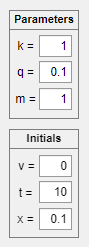
\includegraphics{input.png}}
        \caption{Input variables}
        \label{fig:input}
    \end{minipage}%
    \begin{minipage}{0.625\textwidth}
        \centering
        \shadowbox{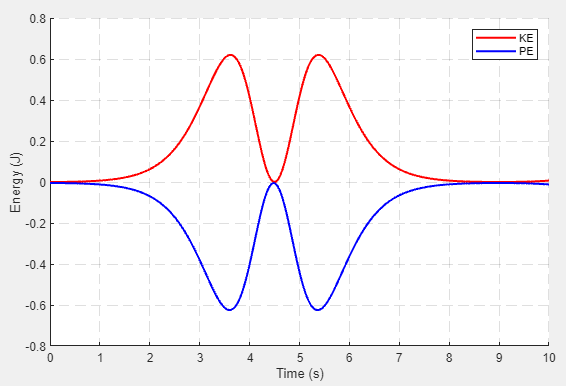
\includegraphics[scale=0.65]{output.png}}
        \caption{Output the result}
        \label{fig:output}
    \end{minipage}
\end{figure}

With the given initial parameters, the MATLAB simulation successfully calculated the kinetic and potential energies of the particle moving under the influence of the conservative force expressed as $F(x) = kx - 4qx^3$. The simulation results matched the theoretical values computed manually, confirming the accuracy of the simulation. Furthermore, we can also replace appropriately many others values of quantities to study other special cases.

\vspace{0.2cm}

This is the user interface for the energy graphing simulation application:

\vspace{-0.25cm}
\begin{figure}[!ht]
  \centering
  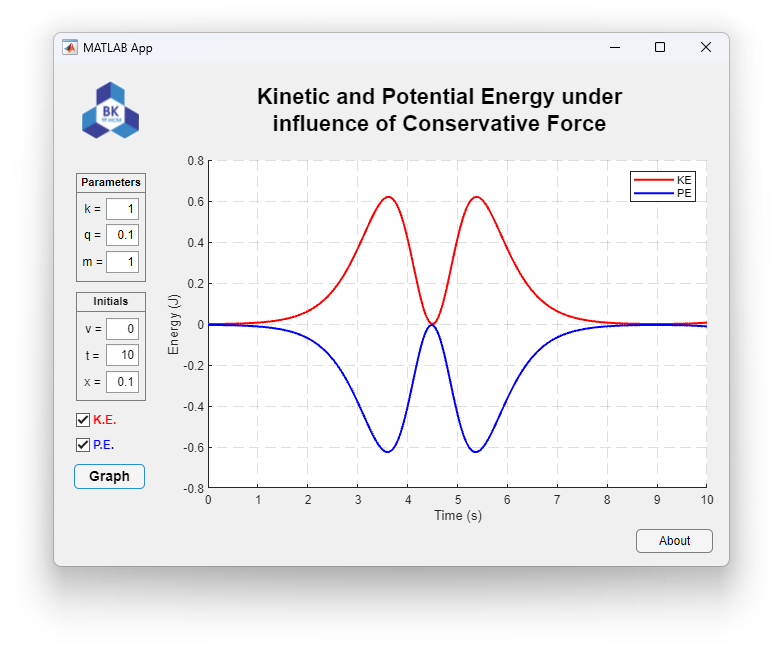
\includegraphics[scale=0.6]{result.png}
  \vspace{-0.75cm}
  \caption{App-based energy graphing simulation}
  \label{fig:result}
\end{figure}

\newpage
By replacing the other initial parameters, we can analyze the state of energy at various points during the motion of an object. For instance, let's change those values by inputting them directly into the app's input fields: $k=2\text{ N/m}$, $q=0.2\text{ N/m}^3$, $m=2\text{ kg}$, $v=1\text{ m/s}$, $t=10\text{ s}$, and $x=0.5\text{ m}$. Then, click the \texttt{Graph} button to observe the plot for the purpose of studying and analyzing it. The resulting plot should resemble the figure below:

\begin{figure}[!ht]
  \centering
  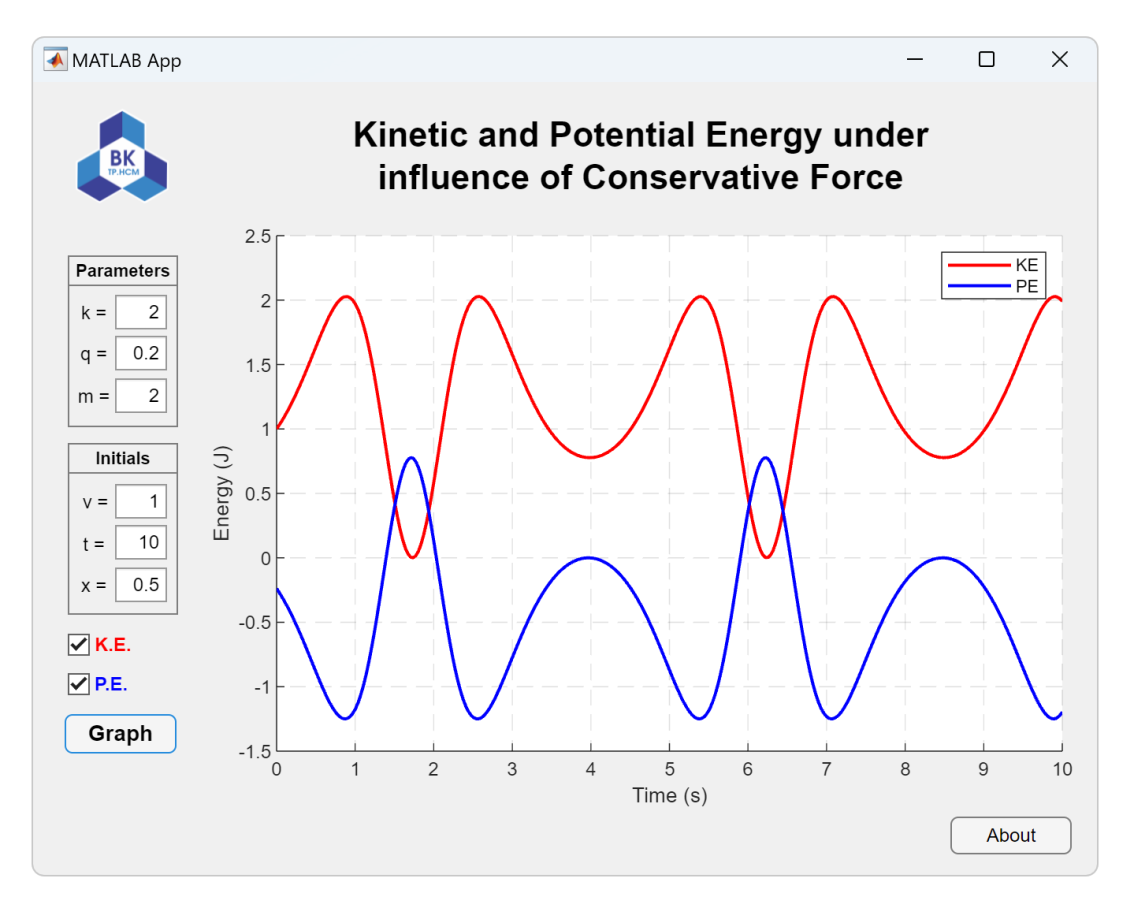
\includegraphics[scale=0.25]{result1.png}
  \vspace{-0.35cm}
  \caption{Another example and the result}
  \label{fig:result}
\end{figure}

\vspace{0.15cm}
Trying out different variables, specifically, $k=3\text{ N/m}$, $q=0.35\text{ N/m}^3$, $m=2\text{ kg}$, $v=5\text{ m/s}$, $t=5\text{ s}$, and $x=5\text{ m}$. The resulting plot may present some difficulty as two wavy plots will stack on top of each other. To address this, users can utilize the \texttt{K.E.} and \texttt{P.E.} checkboxes to control the visibility of kinetic and potential energy, facilitating analysis of the desired plot. The figures below demonstrate the different energy plot visibilities:

\vspace{0.2cm}
\begin{figure}[!htb]
    \centering
    \begin{minipage}{.5\textwidth}
        \centering
        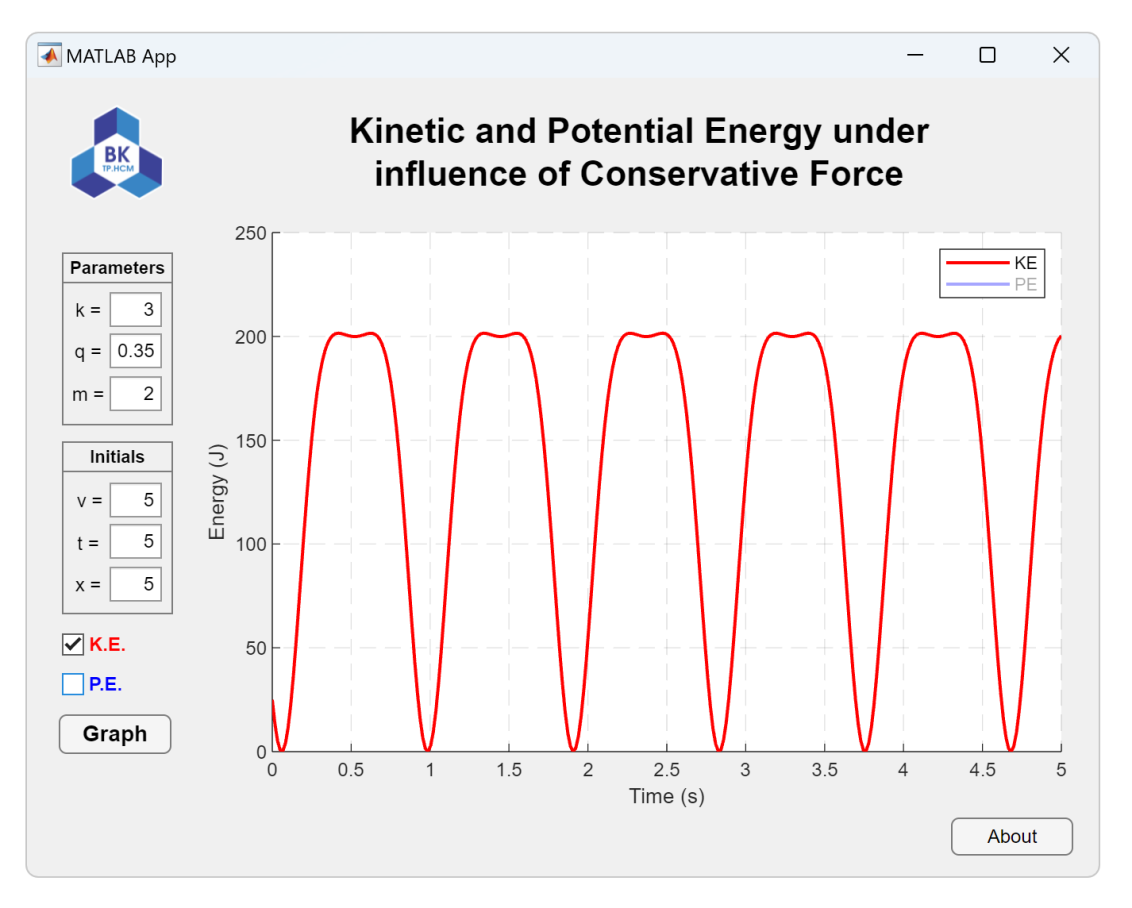
\includegraphics[scale=0.21]{result2_1.png}
  \vspace{-0.75cm}
        \caption{Example with kinetic energy visibility}
    \end{minipage}%
    \begin{minipage}{0.5\textwidth}
        \centering
        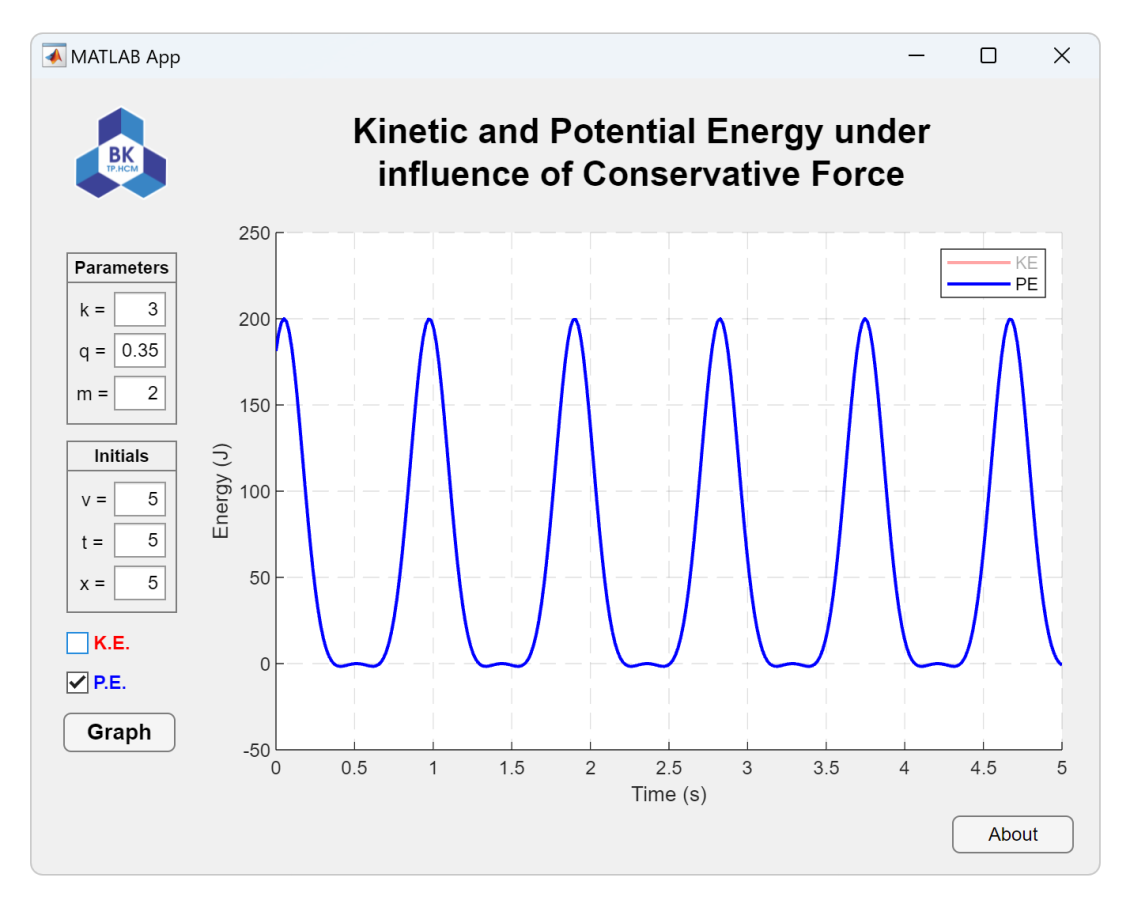
\includegraphics[scale=0.21]{result2_2.png}
  \vspace{-0.75cm}
        \caption{Example with potential energy visibility}
    \end{minipage}
\end{figure}

\newpage
\section{Conclusion}
In conclusion, this MATLAB project demonstrated how to numerically calculate the kinetic and potential energies of a particle moving under the influence of a conservative force. Using the Euler-Cromer method, we were able to accurately compute the motion of the particle and observe that the total energy in the system, which is the sum of kinetic and potential energies, is conserved. The project also allowed us to visualize the changes in kinetic and potential energies over time using MATLAB plots. By adjusting the initial parameters, we were able to explore other special cases and observe how the system behaves under different conditions. Overall, this project provided a valuable insight into numerical methods and their application in solving physical problems.

\newpage
\section{References}
\vspace{0.25cm}
\begin{itemize}[leftmargin=-0.655cm, label=]
    \begin{otherlanguage}{vietnamese}
        \nocite{*}%
        \printbibliography[heading=none]
    \end{otherlanguage}
\end{itemize}
\end{document}